% !TEX program = xelatex
\documentclass[a4paper,11pt]{article}
\usepackage{fontspec,xeCJK,graphicx,amsmath,geometry,booktabs,tabularx,array,float,caption,enumitem,url,hyperref}
\geometry{left=23mm,right=23mm,top=20mm,bottom=22mm}
\setmainfont{texgyretermes-regular.otf}[BoldFont=texgyretermes-bold.otf,ItalicFont=texgyretermes-italic.otf]
\setCJKmainfont{ipaexm.ttf}[AutoFakeBold=1.4]
\newCJKfontfamily\zhfont{gbsn00lp.ttf}
\setmonofont{lmmono10-regular.otf}
\hypersetup{hidelinks,pdfauthor={shigin123},pdftitle={VLMによるブロック操作タスクの実装}}
\urlstyle{same}
\linespread{1.08}
\setlength{\parindent}{1em}
\setlength{\parskip}{0.3em}
\setlength{\tabcolsep}{4pt}
\renewcommand{\arraystretch}{1.15}
\renewcommand{\figurename}{図}
\renewcommand{\tablename}{表}
\captionsetup{font=small,labelfont=bf,labelsep=quad,skip=5pt}
\setlist{nosep,leftmargin=1.6em}
\newcommand{\code}[1]{{\urlstyle{tt}\nolinkurl{#1}}}
\newcolumntype{Y}{>{\raggedright\arraybackslash}X}
\newcommand{\CaseARawBytes}{460}
\newcommand{\CaseAPlanBytes}{631}
\newcommand{\CaseADispatchBytes}{744}
\newcommand{\CaseASamples}{1202}
\newcommand{\CaseADuration}{120.0}
\newcommand{\CaseBRawBytes}{270}
\newcommand{\CaseBPlanBytes}{379}
\newcommand{\CaseBDispatchBytes}{470}
\newcommand{\CaseBSamples}{601}
\newcommand{\CaseBDuration}{60.0}
\newcommand{\PeakTimeOne}{11.8}
\newcommand{\PeakTimeTwo}{32.6}
\newcommand{\PeakTimeThree}{52.2}
\newcommand{\RepeatStateRows}{1 & 0.0--19.8 & (420.000, 100.000, 12.473) & (460.405, 257.748, 22.473) & 160.800 \\
2 & 19.8--39.4 & (460.405, 257.748, 22.473) & (460.326, 257.809, 22.473) & 154.978 \\
3 & 39.4--59.0 & (460.326, 257.809, 22.473) & (460.348, 257.826, 22.473) & 154.988 \\}
\newcommand{\RepeatHandoffMax}{0.000}
\newcommand{\InitialVsSecondDistance}{163.147}
\newcommand{\StackBlue}{(460.622, 81.760, 12.446)}
\newcommand{\StackYellow}{(460.507, 81.792, 37.391)}
\newcommand{\FinalBlue}{(500.163, -296.831, 22.446)}
\newcommand{\FinalYellow}{(500.080, -296.828, 47.391)}
\newcommand{\StackGap}{24.946}
\newcommand{\FinalGap}{24.946}
\newcommand{\RepeatRedDisplacement}{1.863e-09}

\newcommand{\RepeatSimpleRows}{1 & (420.000, 100.000, 12.473) & (460.405, 257.748, 22.473) \\
2 & (460.405, 257.748, 22.473) & (460.326, 257.809, 22.473) \\
3 & (460.326, 257.809, 22.473) & (460.348, 257.826, 22.473) \\}

\begin{document}
\begin{center}
{\Large\bfseries VLMによるブロック操作タスクの実装}\par\vspace{3mm}
Physical AI 応用1講座 最終課題説明資料\\
OmniCampusアカウント名：shigin123\qquad 2026年10月29日
\end{center}

\section{課題の概要と目的}\label{sec:overview}
本課題では，視覚言語モデル（VLM）が画像と自然言語の指示から操作の順番を考え，物理シミュレータ内のロボットアームがその計画を実行するシステムを構築した．目的は，AIの出力を実際の動作へつなぎ，各操作の間で現在の状態を引き継ぎながら，複数段階の作業を完了させることである．

\subsection{実行したタスク}
主な課題は，日本語・英語・中国語が混在する指示による，次の5操作である．赤いブロックは全工程で動かさない条件とした．
\begin{enumerate}
\item 青いブロックをトレーAへ移す．
\item 黄色いブロックをトレーBへ移す．
\item 青いブロックをAの外へ押し出す．
\item 黄色いブロックを青いブロックの上へ積む．
\item 積み重ねた2個を一緒にBへ運ぶ．
\end{enumerate}
さらに，新しく「青を持ち上げて置く操作を3回繰り返す」指示を入力し，同じactionが続く場合にも，更新後の位置から動作を継続できるか確認した．

\subsection{システム構成}
Qwen3-VL-8B-Instructを推論に利用し，Genesis 1.4.4のFranka Pandaモデルで動作を実行した．追加のモデル学習は行っていない．役割の分担を図\ref{fig:flow}に示す．
\begin{figure}[H]\centering\small
\fbox{\parbox[c][12mm][c]{0.18\linewidth}{\centering 画像と指示}}
$\rightarrow$
\fbox{\parbox[c][12mm][c]{0.18\linewidth}{\centering Qwen\\JSON計画}}
$\rightarrow$
\fbox{\parbox[c][12mm][c]{0.18\linewidth}{\centering 対象と引数\\の検査}}
$\rightarrow$
\fbox{\parbox[c][12mm][c]{0.18\linewidth}{\centering 制御プログラム\\Genesis}}
\caption{AIが操作の種類・対象・順番を選び，制御プログラムが位置と関節運動を計算する．}\label{fig:flow}
\end{figure}
\begin{figure}[H]\centering
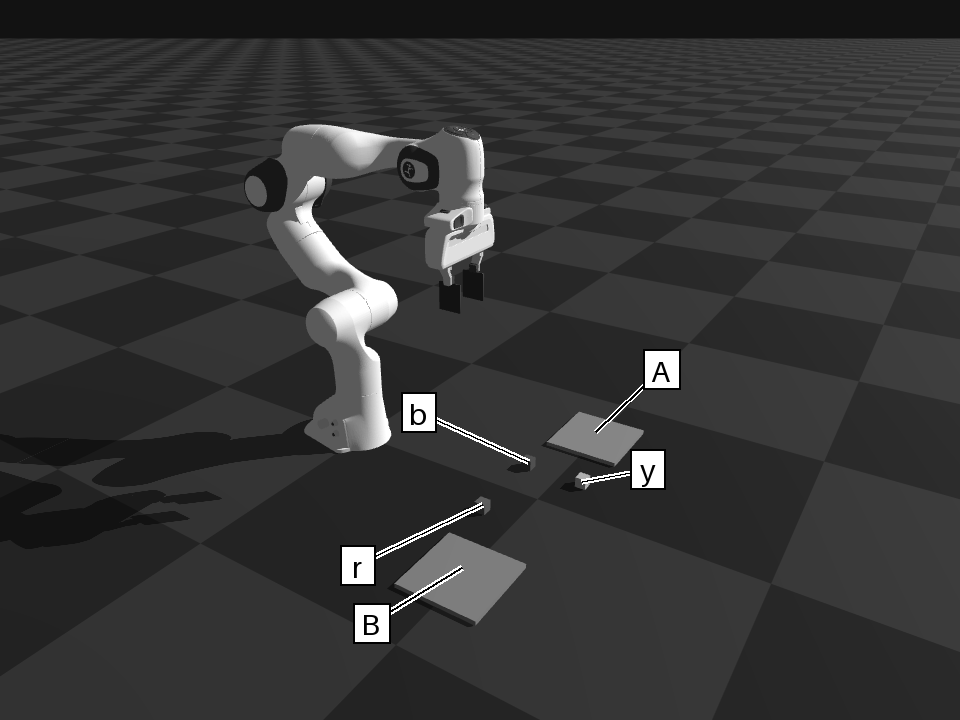
\includegraphics[width=0.50\linewidth]{images/initial.png}
\caption{実際の初期場面を灰度化した画像．b・y・rは青・黄・赤，A・Bはトレーを表す．}\label{fig:initial}
\end{figure}

\clearpage
\section{AIの出力を動作へ渡す仕組み}\label{sec:action}
\subsection{actionの解析}
Qwenには，実際の初期画像，指示全文，物体とトレーのID，使用できる操作を与える．モデルが返すのは関節角度ではなく，例えば次のようなJSONである．
\begin{quote}\small\ttfamily
\{"action":"pick\_place",\\
\phantom{\{}"object\_id":"blue\_block",\\
\phantom{\{}"target\_id":"left\_tray"\}
\end{quote}
これは「青をAへ運ぶ」という意味である．モデルの計画はこのようなactionの配列で，末尾に\code{done}を置く．使用できる操作を表\ref{tab:actions}に示す．
\begin{table}[H]\centering\small
\caption{本課題で使用した操作と，その間をつなぐID．}\label{tab:actions}
\begin{tabularx}{\linewidth}{@{}lYY@{}}\toprule
操作 & 受け渡すID & 動作 \\\midrule
\code{pick_place} & 対象，目的トレー & 持ち上げて置く \\
\code{push_out} & 対象，元のトレー & トレーの外へ押す \\
\code{stack} & 上側の対象，支持物体 & 物体の上へ積む \\
\code{move_stack} & 下側，上側，目的トレー & 2個を一緒に運ぶ \\\bottomrule
\end{tabularx}
\end{table}
受信した文字列を\code{json.loads()}で解析し，動作名，引数，既知のIDを検査する．余分な項目，未知のID，赤を操作・支持物にする指定，末尾の\code{done}がない計画は拒否する．モデル出力をPythonコードとして実行することはない．

\subsection{伝達と状態の更新}
推論プロセスは検査した計画を\code{plan.json}へ保存する．実行側は推論が正常終了したことを確認してから読み込み，再検査したactionを対応する制御関数へ渡す．例えば，上記のIDが\code{pick_place(object_id, target_id)}の引数となる．ファイルは一時ファイルを書いてから置き換え，途中の内容を読み取らないようにした．

操作間で引き継ぐ重要な情報を表\ref{tab:state}に整理する．JSONの計画は最初にまとめて渡し，その後は同じ仮想場面の状態を更新して使う．各actionの終了後に，結果JSONを次の制御関数へ渡す方式ではない．
\begin{table}[H]\centering\small
\caption{actionの指示と，運動計算で使う状態量の区別．}\label{tab:state}
\begin{tabularx}{\linewidth}{@{}p{34mm}YY@{}}\toprule
情報 & 内容 & 次の処理での使い方 \\\midrule
操作と対象ID & 動作名，\code{object_id}などの文字列 & 呼び出す関数と対象物を選ぶ \\
現在の物体位置 & 中心座標$(x,y,z)$，単位m & 次のactionで場面から読み直す \\
手先・関節の目標 & 手先位置，腕7関節と指2自由度 & 逆運動学と位置・力制御で計算する \\
実行状態 & 開始・終了時刻，完了フラグ，終了位置 & 動作と記録を照合する \\\bottomrule
\end{tabularx}
\end{table}
把持時は現在の物体位置から手先目標を作り，Genesisが逆運動学と経路計画を計算する．物体位置にはシミュレータの真値を用い，Qwenが画像から連続関節運動を直接出力する構成ではない．

\clearpage
\section{工夫した点と5段階タスクの結果}\label{sec:original}
\subsection{状態を読み直して操作をつなぐ}
複合操作では，同じ物体を「運ぶ対象」から「積み重ねの支持物」へ切り替える必要がある．そこで，物体の役割をIDで指定し，操作のたびに現在位置を読み直すようにした．例えば，\code{stack}の終了位置と，次の\code{move_stack}が読み取った開始位置は，保存値が一致していた（表\ref{tab:stack}）．
\begin{table}[H]\centering\small
\caption{積み重ね終了から2個搬送へ引き継いだ中心位置．単位mm．}\label{tab:stack}
\begin{tabularx}{\linewidth}{@{}p{18mm}Y@{}}\toprule
物体 & 終了位置＝次の開始位置 $(x,y,z)$ \\\midrule
青 & \StackBlue \\
黄 & \StackYellow \\\bottomrule
\end{tabularx}
\end{table}

\subsection{保護条件と安定した把持}
赤への操作は，指示文だけでなくプログラムでも拒否した．積み重ね前には位置誤差を測り，最大4回・総移動30 mm以内で補正する．指はゆっくり開閉し，2個の同時把持には独自の延長指を用いた．延長指は50×6×60 mm，追加質量19.8 g/指のモデルであり，標準のPanda指とは異なる．物体を指へ固定する拘束は使わず，接触と重力によって動かした．

\begin{figure}[H]\centering
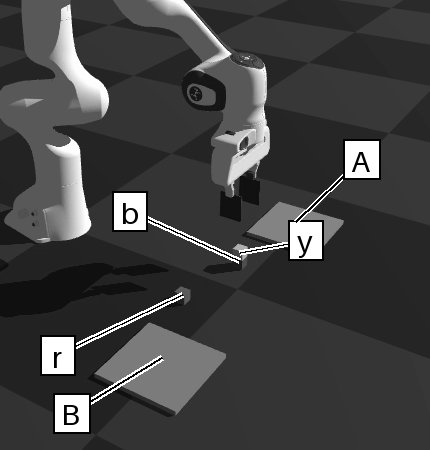
\includegraphics[width=0.38\linewidth]{images/a-stack.png}\hspace{5mm}
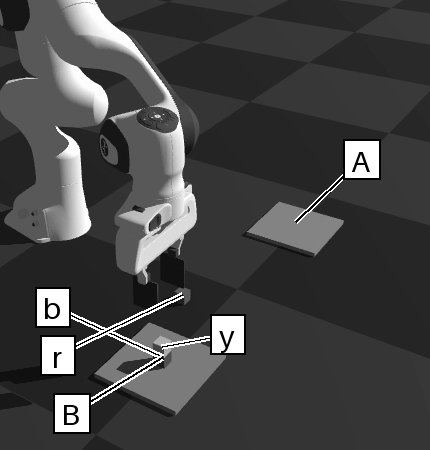
\includegraphics[width=0.38\linewidth]{images/a-final.png}
\caption{同一試行の積み重ね後（左）とBへの配置後（右）．原動画を灰度化し，同じ作業領域を切り出した．注記は保存座標と固定カメラの対応から付けた．}\label{fig:original}
\end{figure}

\subsection{確認できた結果}
5操作を完了し，初期分類，押し出し，積み重ね，搬送中の積層維持，最終配置など7項目の条件を満たした．モデルの\code{done}や見た目だけで判断せず，保存した位置履歴1,202点から再計算した．
\begin{table}[H]\centering\small
\caption{5段階タスクの主要な確認結果．}\label{tab:results}
\begin{tabularx}{\linewidth}{@{}YY@{}}\toprule
確認項目 & 結果 \\\midrule
段階評価 & 7項目すべて達成（正式試行1回） \\
青の押し出し距離 & 175.989 mm \\
2個搬送中の最大水平ずれ & 0.266 mm \\
赤の最大変位 & 0.001 mm未満（シミュレータの数値誤差程度） \\\bottomrule
\end{tabularx}
\end{table}

\clearpage
\section{新しい反復操作と完成した内容}\label{sec:repeat}
\subsection{同じactionを3回繰り返す}
追加した指示は「{\zhfont 抓起蓝色方块然后放下。重复三回}」である．Qwenは青をAへ置く\mbox{\code{pick_place}}を3回生成し，3操作とも実行を完了した．指示には置き先が明記されていないため，Aはモデルが選んだ場所であり，元の位置へ戻したことを示すものではない．

表\ref{tab:repeat}では，第1回の終了位置が第2回の開始位置へ，第2回の終了位置が第3回の開始位置へ引き継がれている．第2回の開始位置は初期位置から約163 mm移動している．同じJSONでも，初期座標を再利用せず，現在位置を読み直すことが必要であった．
\begin{table}[H]\centering\small
\caption{追加した3回反復操作の中心位置．座標の単位はmm．}\label{tab:repeat}
\begin{tabularx}{\linewidth}{@{}>{\centering\arraybackslash}p{8mm}YY@{}}\toprule
回 & 開始位置 $(x,y,z)$ & 終了位置 $(x,y,z)$ \\\midrule
\RepeatSimpleRows
\bottomrule\end{tabularx}
\end{table}
\begin{figure}[H]\centering
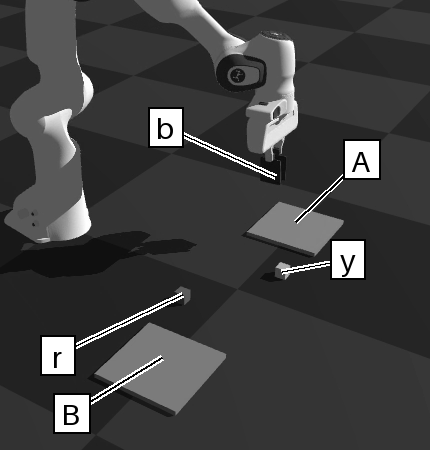
\includegraphics[width=0.28\linewidth]{images/b-lift-1.png}\hfill
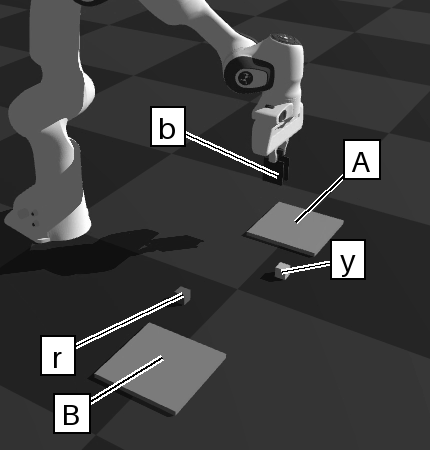
\includegraphics[width=0.28\linewidth]{images/b-lift-2.png}\hfill
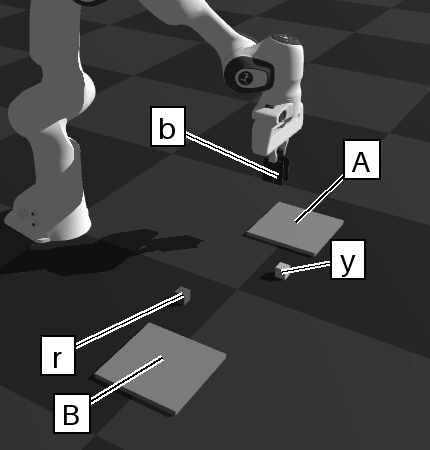
\includegraphics[width=0.28\linewidth]{images/b-lift-3.png}
\caption{左から第1・2・3回の持ち上げ中の実画像．3回とも持ち上げと配置の検査を通過した．}\label{fig:repeat}
\end{figure}

\subsection{完成した内容と適用範囲}
画像・指示からの計画生成，JSONの検査，制御関数への接続，操作後の状態を使った継続動作を実装した．新しい指示にも同じ仕組みを使い，異なる5段階操作と3回反復を実行できた点が本課題の成果である．

検証は固定配置の単純な物体による少数の事例に限られる．追加例は自分で入力した課題のため，5段階課題の採点を流用せず，実行完了と各把持・配置を確認した結果として扱う．未知物体や配置変更，実機での性能，一般的な成功率は未検証である．

\subsection*{提出資料と参照元}
提出動画は5段階タスクの70.5秒で，動作部分の2倍速を明記した．コード，設定，モデル出力，追加した反復操作の記録を公開リポジトリに収録した．
\begin{itemize}\small
\item コード：\url{https://github.com/Fengmc2001/vla-trial-physical-ai-2026}
\item 動画：\url{https://www.youtube.com/watch?v=hS34eNkm5VM}
\item Qwen Team：Qwen3-VL-8B-Instruct（学習済みモデルを利用）．
\item Genesis World：公式の逆運動学・把持例とPandaモデルを参照．基本制御を参考に，課題定義，AI接続，検査，記録・評価を追加した．詳しい帰属はコード内の\code{THIRD_PARTY_NOTICES.md}に示す．
\end{itemize}
\end{document}
